\documentclass[aspectratio=1610]{beamer}
\usepackage[T1]{fontenc}
\usetheme{wildcat}

\usepackage{amsmath,amssymb,amsfonts}
\usepackage{booktabs}
\usepackage{relsize}
\usepackage{pgfplots}
\pgfplotsset{compat=1.16}
%\usepackage[style=verbose,backend=biber]{biblatex}
%\addbibresource{main.bib}
\let\oldfootnotesize\footnotesize
\renewcommand*{\footnotesize}{\oldfootnotesize\tiny}

\def\mathdefault#1{#1}
\everymath=\expandafter{\the\everymath\displaystyle}


\title{Radioactive Decay \\
       {\small\it NE 630 - Lecture 3}}

\date{\input{term.txt} \\ {\footnotesize Git SHA: \input{git_sha.txt}}}

\author{Jeremy Roberts}


\definecolor{ksupurple}{HTML}{512888}
\definecolor{orange}{HTML}{CA7C1B}

\begin{document}

\begin{frame}
\titlepage
\end{frame}
 
 
%%%%%%%%%%%%%%%%%%%%%%%%%%%%%%%%%%%%%%%%%%%%%%%%%%%%
\begin{frame}{Primary Objective}

Students will be able to 

\vfill


\begin{quote}
\textcolor{wcprimary}{determine amounts of a radioactive species and its
daughters in time.}
\end{quote}

\vfill 

\end{frame}

%%%%%%%%%%%%%%%%%%%%%%%%%%%%%%%%%%%%%%%%%%%%%%%%%%%%%%%%%%%%%%%%%%%%%%%%%%%%%%%
\begin{frame}{Review}

Last time, we learned that fission leads to 
\begin{itemize}
 \item 2 large, neutron-rich fragments
 \item 2--3 (prompt) neutrons 
 \item prompt gammas
 \pause
 \item $\beta^{-}$, $\bar{\nu}$, $\gamma$, and even n's from 
    the decay of fission fragments and their daughters.
\end{itemize}
The latter decays drive much of the heat produced in spent fuel.

\vfill 
\pause 

{\bf Concept Check}: Why are the two fragments ``neutron rich?''
 

\end{frame}

%%%%%%%%%%%%%%%%%%%%%%%%%%%%%%%%%%%%%%%%%%%%%%%%%%%%%%%%%%%%%%%%%%%%%%%%%%%%%%%
\begin{frame}{Review}

 
Moreover, if we put $n_0$ neutrons into a fissile system, and at least one induces fission, we can define
the {\bf multiplication factor}
\begin{equation*}
 k = \frac{\text{\# n's in generation i}}{\text{\# n's in generation i - 1}}
\end{equation*}

\vfill % pushes the block to the bottom
 
\begin{columns}[T,onlytextwidth]
  %--- Left: equations -----------------------------------------------
  \begin{column}{0.46\textwidth}
    If $k$ is fixed and $\ell$ is the {\bf neutron lifetime}, then
    \[
      \frac{n(t)}{n(0)} = k^{t/\ell}.
    \]
    and, if $k \approx 1$,
    \[
    n(t) \approx n_0  e^{\left(\frac{k-1}{\ell}\,t\right)}.
    \]
  \end{column}

 % --- Right: small PGFPlots figure -----------------------------------
  \begin{column}{0.54\textwidth}
    \begin{tikzpicture}
      \begin{axis}[
        width=\linewidth,
        height=0.46\textheight,
        xmin=0, xmax=6,
        ymin=0, ymax=5,
        grid=both,
        xlabel={$t/\ell$},
        ylabel={$n(t)/n(0)$},
        ticklabel style={font=\scriptsize},
        label style={font=\scriptsize},
        legend style={draw=none, font=\scriptsize, at={(0.7,0.97)}, anchor=north east}
      ]
        \addplot+[thick, mark=none, samples=100, domain=0:6, color=ksupurple]
          {exp(ln(1.20)*x)}; % = (1.20)^(t/ell)
        \addlegendentry{$k=1.20$ (supercritical)}

        \addplot+[thick, dotted, mark=none, domain=0:6, color=black]
          {1};
        \addlegendentry{$k=1.00$ (critical)}

        \addplot+[thick, dashed, mark=none, samples=100, domain=0:6, color=orange]
          {exp(ln(0.80)*x)}; % = (0.80)^(t/ell)
        \addlegendentry{$k=0.80$ (subcritical)}
      \end{axis}
    \end{tikzpicture}
  \end{column}
\end{columns}

\vfill
 
{\bf Back-of-the-Envelope}: If $l = 10^{-4}$ s and $n_0 = 1$, how much energy (in J)
is produced in 1 s if $k = 1.0001$?  How about if $k=1.01$?


\end{frame}

%%%%%%%%%%%%%%%%%%%%%%%%%%%%%%%%%%%%%%%%%%%%%%%%%%%%%%%%%%%%%%%%%%%%%%%%%%%%%%%
\begin{frame}{A Summary of Radioactive Decay}

Given a sample of $N(t)$ nuclei of a radioactive species at some time $t$, we expect the number of 
decays $\Delta N$ in a period of time $\Delta t$ to be
\begin{equation*}
 \Delta N = - \lambda N \Delta t \pause \quad \longrightarrow \quad \boxed{\frac{dN}{dt}=-\lambda N(t)} \, ,
\end{equation*}
where $\lambda = \log{2}/t_{1/2}$ is


The {\bf activity} of the sample $A(t) = \lambda N(t)$ is the {\it rate at which nuclei are lost}.

\pause 
\vfill 

We can also model $N(t)$ when nuclei are added a rate $R(t)$:
\begin{equation*}
 \boxed{\frac{dN}{dt}=-\lambda N(t) + R(t)} \, .
\end{equation*}

\pause 
\vfill

How do we solve these equations?

\end{frame}


%%%%%%%%%%%%%%%%%%%%%%%%%%%%%%%%%%%%%%%%%%%%%%%%%%%%%%%%%%%%%%%%%%%%%%%%%%%%%%%
\begin{frame}{Example: Decay Chain}

Among possible fission products is ${}^{94}\text{Sr}$, which decays to
the stable ${}^{94}\text{Zr}$ via

\[
{}^{94}_{38}\mathrm{Sr}
  \;\xrightarrow[\;75~\text{s}\;]{\;\beta^-\;}
{}^{94}_{39}\mathrm{Y}
  \;\xrightarrow[\;18.7~\text{min}\;]{\;\beta^-\;}
{}^{94}_{40}\mathrm{Zr} \, .
\]

Assume that $N_{\text{Sr}}(0) = N_0$, $N_{\text{Y}}(0) = 0$, and  $N_{\text{Zr}}(0) = 0$.  Then

\begin{enumerate}
 \item write down the set of equations that model this decay chain.
 \item determine $N_{\text{Sr}}(t)$, $N_{\text{Y}}(t)$, and $N_{\text{Zr}}(t)$.
\end{enumerate}




\end{frame}


 




\end{document}

